\documentclass[mathNotesPreamble]{subfiles}
\begin{document}
%\relscale{1.4} %TODO
\section{13.6: Cylinders and Quadric Surfaces}
  \textbf{Cylinders and Traces:}\\
    When talking about three-dimensional surfaces, a \textit{cylinder} refers to a surface that is parallel to a line. When considering surfaces that is parallel to one of the coordinate axes, that the associated variable is missing (e.g. $3y^2+z^2=8$ is parallel to the $x$-axis).
  
  \begin{defn*}[Trace]
    A \textbf{trace} of a surface is the set of points at which the surface intersects a plane that is parallel to one of the coordinate planes. The traces in the coordinate planes are called the \textbf{$xy$-trace}, the \textbf{$yz$-trace}, and the \textbf{$xz$-trace} (Figure 13.80).
  \end{defn*}
  \begin{center}
    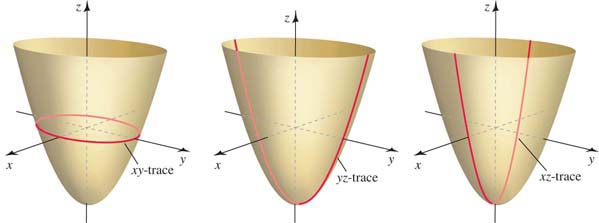
\includegraphics[width=0.7\linewidth]{images/briggs_13_06/fig13_80}
  \end{center}

  \begin{ex*}
    Roughly sketch the following functions:
    \begin{enumerate}
      \item $x^2+4y^2=16$
      \item $x-\sin(z)=0$
    \end{enumerate}
  \end{ex*}
  \vspace*{\stretch{1}}

  \begin{center}
    \begin{tikzpicture}
      \begin{axis}[
        axis lines=center,
        axis line style={black,->},
        xmin=-1, xmax=6.5,
        ymin=-1, ymax=6.5,
        zmin=-1, zmax=6.5,
        xmajorticks=false,
        ymajorticks=false,
        zmajorticks=false,
        enlargelimits={abs=0.75},
        view={125}{25},
        every axis plot/.append style={line width=0.5pt, color=blue}
        ]
      \end{axis}
    \end{tikzpicture}
    \hspace*{0.1\textwidth}
    \begin{tikzpicture}
      \begin{axis}[
        axis lines=center,
        axis line style={black,->},
        xmin=-1, xmax=6.5,
        ymin=-1, ymax=6.5,
        zmin=-1, zmax=6.5,
        xmajorticks=false,
        ymajorticks=false,
        zmajorticks=false,
        enlargelimits={abs=0.75},
        view={125}{25},
        every axis plot/.append style={line width=0.5pt, color=blue}
        ]
      \end{axis}
    \end{tikzpicture}
  \end{center}
  \pagebreak

  \textbf{Quadric Surfaces:}\\
    \textbf{Quadric surfaces} are described by the general quadratic (second-degree) equation in three variables,
      \[Ax^2+By^2+Cz^2+Dxy+Exz+Fyz+Gx+Hy+Iz+J=0,\]
    Where the coefficients $A,\dots,J$ and not all zero. To sketch quadric surfaces, keep the following ideas in mind:
    \begin{enumerate}
      \item \textbf{Intercepts} Determine the points, if any, where the surface intersects the coordinate axes. To find these intercepts, set $x$, $y$, and $z$ equal to zero in pairs in the equation of the surface, and solve for the third coordinate.
      \item \textbf{Traces} Finding traces of the surface helps visualize the surface. Setting $x$, $y$, and $z$ equal to zero in pairs gives the planes parallel in that pair's plane.
      \item \textbf{Completing the figure} Sketch some traces in parallel planes, then draw smooth curves that pass through the traces to fill out the surface.
    \end{enumerate}

    \begin{ex*}[An ellipsoid]
      The surface defined by the equation $\displaystyle \frac{x^2}{a^2}+\frac{y^2}{b^2}+\frac{z^2}{c^2}=1$. Graph $a=3$, $b=4$ and $c=5$.
    \end{ex*}
    \vspace*{\stretch{1}}
    \pagebreak

    \begin{ex*}[An elliptic parabaloid]
      The surface defined by the equation $\displaystyle z=\frac{x^2}{a^2}+\frac{y^2}{b^2}$. Graph the elliptic paraboloid with $a=4$ and $b=2$.
    \end{ex*}
    \vspace*{\stretch{1}}
    \pagebreak

    \begin{ex*}[A hyperboloid of one sheet]\mbox{}\\
      Graph the surface defined by the equation $\displaystyle \frac{x^2}{4}+\frac{y^2}{9}-z^2=1$.
    \end{ex*}
    \vspace*{\stretch{1}}
    \pagebreak
    
    \begin{ex*}[A hyperboloid of two sheets]
      Graph the surface defined by the equation $-16x^2-4y^2+z^2+64x-80=0.$
    \end{ex*}
    \vspace*{\stretch{1}}
    \pagebreak

    \begin{ex*}[Elliptic cones]
      Graph the surface defined by the equation $\displaystyle \frac{y^2}{4}+z^2=4x^2$.
    \end{ex*}
    \vspace*{\stretch{1}}
    \pagebreak

    \begin{ex*}[A hyperbolic paraboloid]\mbox{}\\
      Graph the surface defined by the equation $\displaystyle z=x^2-\frac{y^2}{4}$. 
    \end{ex*}
    \vspace*{\stretch{1}}
    \pagebreak

    
  
  \begin{center}
  %https://tex.stackexchange.com/questions/337570/tabularx-with-different-column-widths
    \renewcommand{\tabularxcolumn}[1]{m{#1}} %sets columns to vertically centered
    \relscale{0.775}
    \begin{tabularx}{\linewidth}{@{}
      >{\hsize=0.25\hsize}X@{\hspace*{20pt}}
      >{\hsize=0.45\hsize}X
      >{\hsize=0.725\hsize}X
      >{\hsize=0.4\hsize}Y@{}}\toprule
      \textbf{Name}& 
      \textbf{Standard Equation}& 
      \multicolumn{1}{c}{\textbf{Features}}&
      \textbf{Graph}\\\midrule
      %
      Ellipsoid& 
      $\displaystyle \frac{x^2}{a^2}+\frac{y^2}{b^2}+\frac{z^2}{c^2}=1$& 
      All traces are ellipses.& 
      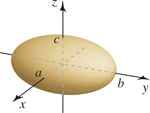
\includegraphics[width=0.25\linewidth]{images/briggs_13_06/tab13_1_fig1}\\
      %
      Elliptic paraboloid& 
      $\displaystyle z=\frac{x^2}{a^2}+\frac{y^2}{b^2}$& 
      Traces with $z=z_0>0$ are ellipses. Traces with $x=x_0$ or $y=y_0$ are parabolas.& 
      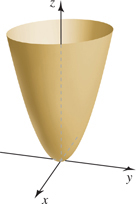
\includegraphics[width=0.25\linewidth]{images/briggs_13_06/tab13_1_fig2}\\
      %
      Hyperboloid of one sheet& 
      $\displaystyle \frac{x^2}{a^2}+\frac{y^2}{b^2}-\frac{z^2}{c^2}=1$& 
      Traces with $z=z_0$ are ellipses for all $z_0$. Traces with $x=x_0$ or $y=y_0$ are hyperbolas.& 
      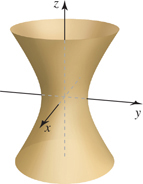
\includegraphics[width=0.25\linewidth]{images/briggs_13_06/tab13_1_fig3}\\
      %
      Hyperboloid of two sheets& 
      $\displaystyle -\frac{x^2}{a^2}-\frac{y^2}{b^2}+\frac{z^2}{c^2}=1$&
      Traces with $z=z_0$ with $\abs{z_0}>\abs{c}$ are ellipses. Traces with $x=x_0$ and $y=y_0$ are hyperbolas.& 
      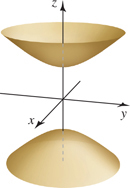
\includegraphics[width=0.25\linewidth]{images/briggs_13_06/tab13_1_fig4}\\
      %
      Elliptic cone& 
      $\displaystyle \frac{x^2}{a^2}+\frac{y^2}{b^2}=\frac{z^2}{c^2}$& 
      Traces with $z=z_0\neq0$ are ellipses. Traces with $x=x_0$ or $y=y_0$ are hyperbolas or intersecting lines.& 
      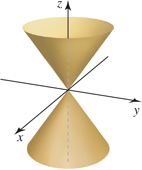
\includegraphics[width=0.25\linewidth]{images/briggs_13_06/tab13_1_fig5}\\
      %
      Hyperbolic paraboloid& 
      $\displaystyle z=\frac{x^2}{a^2}-\frac{y^2}{b^2}$& 
      Traces with $z=z_0\neq0$ are hyperbolas. Traces with $x=x_0$ or $y=y_0$ are parabolas.& 
      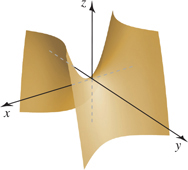
\includegraphics[width=0.3\linewidth]{images/briggs_13_06/tab13_1_fig6}\\
      %
      \bottomrule
    \end{tabularx}
  \end{center}
  \pagebreak
  
\end{document}